\subsection{Why virtualized HPC?}
Although HPC workloads are most often run on bare-metal systems, this has started to change 
with the realization that many of the benefits that virtualization offers to enterprises 
can often also add value in HPC environments~\cite{mergen2006virtualization,nagarajan2007proactive,simons2010virtualizing}. The following are among those benefits:
\begin{itemize}
	\item Supports a more diverse end-user population with differing software requirements 
        on the same platform
	\item Provides multi-tenancy data security by isolating user workloads into separate VMs and virtual networks
	\item Offers fault isolation, root access, and other capabilities not available in traditional HPC environments
	\item Creates a more dynamic execution environment in which VMs and their encapsulated workloads 
	can be live-migrated across the cluster for load balancing, for maintenance, for fault avoidance, and so on
\end{itemize}

In the context of cloud computing, virtualization can refer to either hypervisor-based full virtualization or container-based OS virtualization. However, container-based virtualization not only lacks support of OS 
heterogeneity, but also falls short in providing the same level of security isolation 
and may incur higher performance interference with respect to full virtualization~\cite{reshetova2014security,sharma2016containers}. Therefore, we will focus on hypervisor-based full virtualization in the remainder of this paper. 

In addition to the above benefits, the performance of HPC applications on virtual platforms has dramatically 
improved over the past years~\cite{luszczek2011evaluation,younge2011analysis,morabito2015hypervisors}. This is especially true for HPC throughput workloads, which in contrast to Message Passing Interface (MPI) workloads, 
consist of a large number of independent tasks that can execute in parallel. Throughput workloads represent a 
significant portion of HPC workloads and include financial services, life sciences, electronic design automation, image rendering, etc. 
Studies have demonstrated that the performance gap between virtual and bare-metal for HPC throughput workloads has 
closed, with just 1 or 2 percentage difference~\cite{michael2018overcommit}. 
%as shown in Figure \ref{fig:perf_gap}~\cite{michael2018overcommit}.

% \begin{figure}[!t]
%    \begin{center}
%        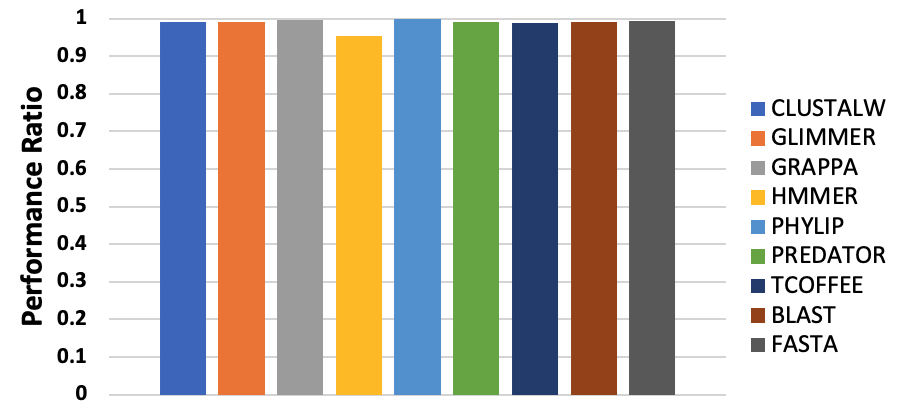
\includegraphics[width=\columnwidth]{Figures/perf_gap}
%    \end{center}
%    \caption{Performance ratio between virtual and bare-metal for a set of life sciences workloads 
%    from BioPerf benchmark suite~\cite{1526013}. Higher is better. VMware ESXi 5.5 is used as the hypervisor.}
%    \label{fig:perf_gap}
%  \end{figure}

\subsection{HPC cloud resource allocation}
Virtualization brings new flexibility to HPC. With this flexibility, however, one must be careful to configure 
the cloud environment to simultaneously achieve both agility and performance.
Although it is possible to create a single virtual cluster (VC) that spans the entire HPC partition in a data center 
with one maximally sized VM per node to serve all the HPC tenants, this approach misses the opportunity to enable several important 
virtualization benefits. Among these are the ability to support per-tenant or per-project software stacks as well 
as security and fault separation between the tenant workloads. In the more typical case, multiple VCs should be hosted simultaneously on the physical cluster for flexibility and for isolation between tenants.

In a situation in which a tenant is using resources intensively, it might make most sense to assign 
a dedicated subset of hardware to the tenant and to appropriately configure VMs on those nodes. 
With two such tenants, one can either place their VMs on a non-overlapping set of nodes (Figure~\ref{fig:allocation1}), 
or place them on the same nodes, being careful to size their VMs to avoid any over-commitment (Figure~\ref{fig:allocation2}). 
%Typically, the size of each such VM is set to the number of cores available in each underlying physical CPU to take 
%advantage of the hardware NUMA topology. 
%This approach works well if the VMs are so heavily loaded that 
%few cycles are left unused on each node. However, it is often the case that such projects do not in actuality 
%show this degree of resource intensity. Although they might be very busy and resource constrained in some 
%time periods, they can also be less busy and even idle in other periods. In such cases, sizing VMs as 
%described--so that they partition the available physical cores--can lead to commensurate losses in 
%throughput because the idle CPUs serving one VM are not available to the other busy VM.
The major flaw with these approaches is that resources are statically partitioned and thus susceptible to under-utilization. 
Although tenants might be very busy during some 
time periods, they can also be less busy and even idle during other periods. In such cases, sizing VMs as 
described above can lead to commensurate losses in 
throughput because the idle resources serving one VM are not available to the other busy VMs.

\begin{figure}
     \centering
     \begin{subfigure}[b]{0.45\textwidth}
         \centering
         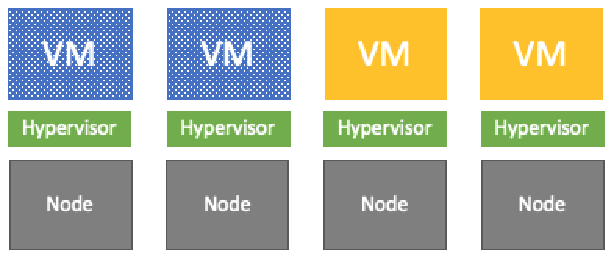
\includegraphics[width=\textwidth]{Figures/allocation1.pdf}
         \caption{Partition on non-overlapping nodes}
         \label{fig:allocation1}
     \end{subfigure}
     \hfill
     \begin{subfigure}[b]{0.45\textwidth}
         \centering
         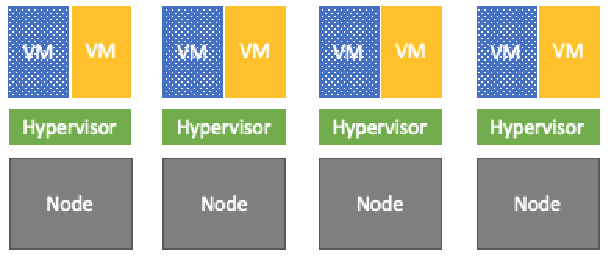
\includegraphics[width=\textwidth]{Figures/allocation2.pdf}
         \caption{Partition on same nodes}
         \label{fig:allocation2}
     \end{subfigure}
     \caption{Example of traditional static allocation with four hosts and two tenants. Blue VMs for one tenant and yellow VMs for the other. Width of a VM box represents
     the fraction of cores assigned to that VM.}
     \label{fig:static_allo}
\end{figure}

\subsection{Resource over-commitment}
The key to avoiding the above resource waste issue is resource over-commitment. In a 
virtualized environment, resource over-commitment means configuring VMs with more virtual resources than the available 
physical ones. For example, on a host with 4 CPU cores and 8 GB memory, one could create two VMs each 
with 4 virtual CPUs and 6 GB virtual memory. 

CPU over-commitment is accommodated by multiplexing virtual 
CPUs onto physical CPUs. In a modern hypervisor like VMware ESXi, a shares-based mechanism can be enabled  
in the scheduler so that VMs with different shares get different portions of the physical CPUs, 
even in the case of CPU over-commitment. %~\cite{vmware2013scheduler}. 
Furthermore, a work-conserving scheduler 
allows one VM to consume more than its fair CPU shares if there are idle cycles from other VMs. 
Memory over-commitment, on the other hand, is more challenging since multiplexing is not 
applicable. It is achieved by applying a set of memory reclamation techniques, including transparent page sharing (TPS), 
ballooning, compression, and hypervisor swapping~\cite{Waldspurger:2002:MRM:844128.844146,banerjee2013memory}. These techniques differ in the incurred 
overhead and are individually controlled by the hypervisor based on system memory state.  

Resource over-commitment has been studied in the literature, but previous works either only consider CPU over-commitment, or they do not optimize specifically for HPC workloads~\cite{tran2019,Tesfatsion2018,shao2011analyzing,gordon2011ginkgo,li2012evaluating}. For example, while~\cite{li2012evaluating} only presents some preliminary memory over-commitment tests using a dummy memory allocation program, \cite{gordon2011ginkgo} adapts memory allocation in a memory over-committed setting by optimizing a 
pre-defined fine-grained performance metric, such as instructions per cycle, which is not commonly available in HPC applications.



